\section{Estimation of Charge Mis-Identification (Type-I)}
\label{sec:chargemisid}

In order to understand the Type-I background, we need to know the 
probability as a function of $P_T$ and $\eta$ for an electron
to have its charge misassigned (flipped).  We called this 
probability the ``charge-flip rate'', $P_{ChargeFlip}$.


The sample of $Z \to ee$ is an ideal sample to measure the charge-flip rate.
However, the $P_T$ range of electrons from $Z$ decays is limited
to (roughly) 20 GeV $< P_T <$ 60 GeV, while we need the flip-rate
down to 10 GeV and up to higher momenta.
Our plan then is to measure $P_{chargeFlip}$ from $Z$ data in the 
accessible $P_T$ range;  we will then compare 
the $P_{chargeFlip}$ from $Z$ data with the $P_{chargeFlip}$ from 
Monte Carlo using a single electron gun.  In the analysis we will
use the Monte Carlo flip rate, possibly adjusted if we find that
data and Monte Carlo do not agree


In this Section we demonstrate that we are able to extract 
$P_{chargeFlip}$ from a Monte Carlo Drell Yan sample, and that
this flip rate agrees with the flip rate from a 
single electron gun.  The analysis described here is based on 
a dielectron sample within the $Z$ mass region
($76 < m_{ee} < 106 $ GeV).   No opposite sign requirement is 
made.  Both electrons must pass all the identification and isolation
criteria described in Section~\ref{sec:eventselection}.



\subsection{Measurement of charge-flip rate on $Z$ events}

We define the charge-flip rate as

\begin{equation}
P_{ChargeFlip} = \frac{N_{Wrong}(P_T, |\eta|)}{N_{Total}(P_T, |\eta|)}
\end{equation}

where $N_{Wrong}(P_T, |\eta|)$ is the number of wrongly charged electrons  
and $N_{Total}(P_T, |\eta|)$ is 
the total number of electrons in the sample. We select events with same sign $(SS)$ 
and opposite sign $(OS)$ dielectrons within the $Z$ mass range, with both electrons passing the 
selection described in Section~\ref{sec:electron}.

We determine $P_{ChargeFlip}$ in two steps.  In the first step we limit ourselves
to the barrel region, $|\eta| < 1.0$, where we expect $P_{ChargeFlip}$ to have 
a small $\eta$ dependence.  Thus, we select $Z \to ee$, same sign (SS) as well as
opposite sign (OS), with both electrons in the barrel.  
We construct two $P_T-|\eta|$
distributions, one for electrons in the SS sample and 
one for electrons in the OS samples.  Neglecting the small 
probability of double charge flips, the OS distribution will contain only
electrons with the correct charge assignment, while the SS distribution
will contain a 50-50 admixture of charge flipped and non-charge flipped
electrons.  Then, 
the number of wrongly charged electrons in the barrel as a function
of $P_T$ and $|\eta|$ is obtained as

\begin{equation}
  N_{Wrong}(P_T, |\eta|) = SS(P_T, |\eta|) - k * OS(P_T, |\eta|) 
\end{equation}

The normalization $k$ is given by the ratio of SS and OS events.
The charge-flip rate in the barrel is then obtained by dividing 
$N_{Wrong}(P_T, |\eta|)$ by the total number of electrons as a 
function of $P_T$ and $|\eta|$.

Once $P_{ChargeFlip}$ in the barrel has been determined, the second step
of the procedure is to extend the measurement to higher rapidities 
($|\eta|>1$).  This is done using $Z \to ee$, OS as well as SS, with 
one electron of $|\eta|<1$ and one electron of $|\eta|>1$.  
$P_{ChargeFlip}$ for $|\eta|>1$ is determined by taking the ratio
of the $P_T-|\eta|$ distributions of electrons with 
$|\eta|>1$ in the SS sample to the total.  A correction needs to 
be applied to account for the events with the charge of the
$|\eta|<1$ flipped.  This is done using the  $P_{ChargeFlip}$
for $|\eta|<1$ determined in the first step.


\begin{figure}[htb]
\begin{center}
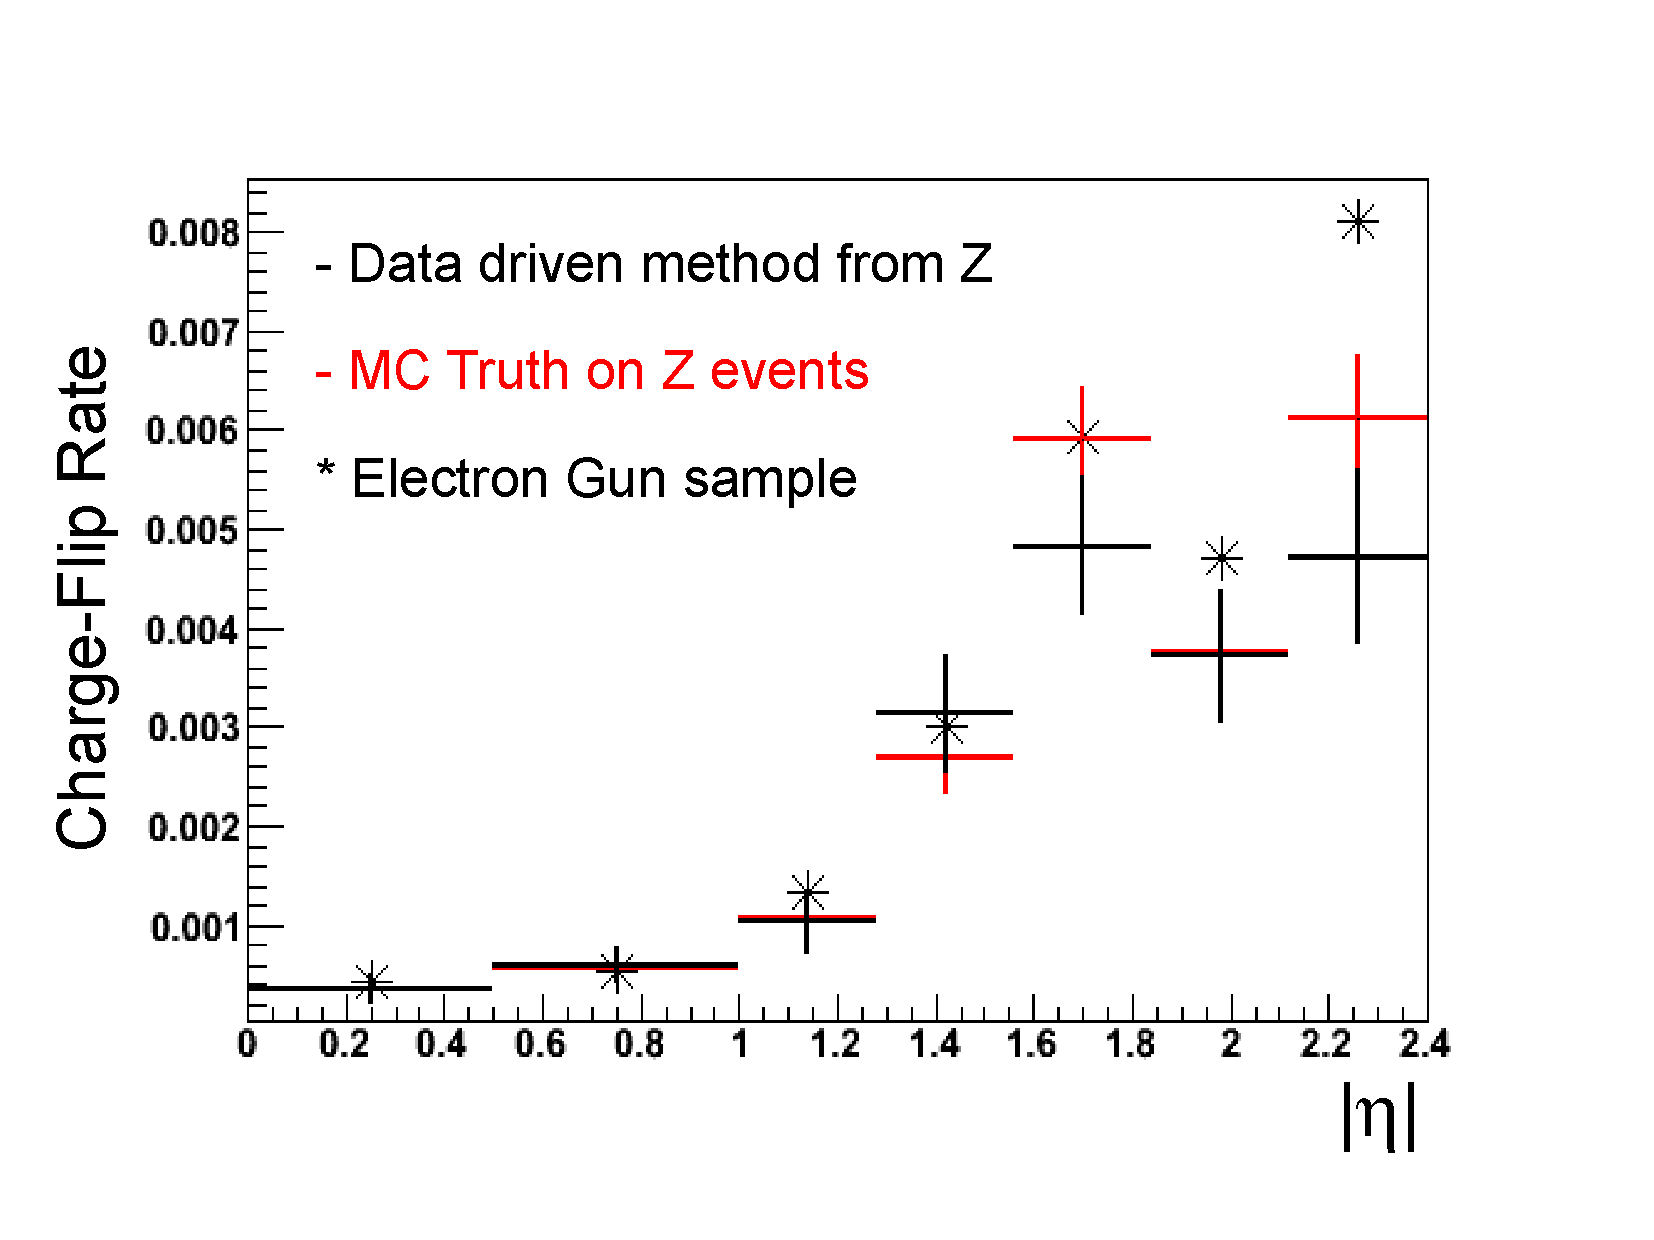
\includegraphics[width=0.7\linewidth]{figs/fr_rate.pdf}
\caption{Charge-flip rate as a function $|\eta|$ for the ``electron gun'' sample (star) compared with 
distributions using data driven method from $Z$ (black histograms) as well as truth matched $Z$ events 
(red histogram).
The integrated uminosity of the $Z$ sample is about 300 pb$^{-1}$.  
\label{fig:charge_fliprate}}
\end{center}
\end{figure}


It is important to verify that this procedure yields the correct 
charge-flip rate.  To this end, in Figure~\ref{fig:charge_fliprate}
we compare three flip rates as a function of $|\eta|$ and integrated
over $P_T$:
\begin{enumerate}
\item The flip rate obtained from the $Z$ sample using the two-step
procedure outlined above.
\item The flip rate obtained from the $Z$ sample using MC truth.
\item The flip rate obtained from the single electron gun, weighted by the
$P_T-\eta$ distribution of electrons in the $Z$ sample.
\end{enumerate}
The three distributions agree quite well. This demonstrates that 
we are able to measure the flip rate from the data in the $P_T$
region covered by $Z \to ee$. 


\subsection{Application of charge-flip rate to our analysis}

We now perform a test of the charge flip prediction on \ttbar MC events by relaxing cuts on \met and jets. The test is meant
to demonstrate that the charge-flip rate as determined from the ``electron gun'' sample can be applied
to \ttbar events. Dilepton events are selected without any \met and jet cuts using an integrated 
luminosity of 100 pb$^{-1}$. The observed event yield is obtained by selecting same sign dielectron events.
In order to get the estimation we use the following procedure:

\begin{itemize}
\item Select opposite sign dielectrons using the standard selection.
\item Obtain the $P^1_{ChargeFlip}$ and  $P^2_{ChargeFlip}$ for each electron for a given $p_T$ and $\eta$.
We use the charge-flip rate from the electron gun.
\item Assuming either of the electrons can flip signs, the flip probability is given by $ F = P_{ChargeFlip}/(1 - P_{ChargeFlip})$.
\item Weight each event by $weight * (F^1 + F^2)$.
\item Add up all of the weights
\end{itemize} 
Results of the Monte Carlo tests for event yields is given in Table~\ref{tab:ChFlip_Test}. From this study we 
can conclude that the charge-flip rate does a very good job of reproducing the rate of charge mis-identification
of electrons in \ttbar events.  
\begin{table}[hbt]
\begin{center}
\begin{tabular}{|l|c|}\hline
Sample & Event yield \\ \hline
\ttbar (Observed) & 2.4 $\pm$ 0.3 \\
\ttbar (Predicted) & 2.1 \\
\hline
\end{tabular}
\caption{ Monte Carlo test of the electron charge-flip rate.  Rates are normalized to 100 pb$^{-1}$ of integrated luminosity. \label{tab:ChFlip_Test}}
\end{center}
\end{table}

We are now ready to apply the charge-flip rate to our \ttbar sample after the full analysis selection. 
The same sign dilepton sample will have 
three different contributions from Type-I, Type-II and Type-III events. The results of the application of 
the procedure outlined above is summarized in Table~\ref{tab:ChFakePredict}.
\vspace{2mm}
\begin{table}[hbt]
\begin{center}
\begin{tabular}{|l|c|c|c|c|c|c|}\hline
Same Sign leptons & Total &      Type-I &  Type-II & Type-II a) & Type-II b) & Type-III \\ \hline
$ee$ (predicted) 	 & 0.05 & 	0.05 &	0.00 &	0.00 &	0.00 &	0.00 \\
$\mu\mu$ (predicted)     & 0.00 &	0.00 &	0.00 &	0.00 &	0.00 &	0.00 \\
$e\mu$ (predicted)	 & 0.07 &	0.07 &	0.00 &	0.00 &	0.00 &	0.00 \\
total (predicted) 	 & 0.12 &	0.12 &	0.00 &	0.00 &	0.00 &	0.00 \\
\hline
\end{tabular}
\caption{ The number of events predicted using charge-flip rate in \ttbar events for various types. Rates are normalized 
to 100 pb$^{-1}$.\label{tab:ChFakePredict}}
\end{center}
\end{table}

Using Table~\ref{tab:fakeOrigin} as observed and Table~\ref{tab:ChFakePredict} as the 
prediction, we find that the charge-flip method predicts the bulk of the Type-I events.
Out of a total of $0.22 \pm 0.10$ (roughly corresponds to 5 MC events) expected events, we predict 
$0.12$ ($\approx 3$) events in 100 pb$^{-1}$. As expected,
the method does not predict any contribution from Type-II events. 
We consider the agreement to be satisfactory.

